\documentclass{ximera}
 
%% You can put user macros here
%% However, you cannot make new environments

\listfiles

\graphicspath{{./}{firstExample/}{secondExample/}}

\usepackage{tikz}
\usepackage{tkz-euclide}
\usepackage{tikz-3dplot}
\usepackage{tikz-cd}
\usetikzlibrary{shapes.geometric}
\usetikzlibrary{arrows}
\usetikzlibrary{decorations.pathmorphing,patterns}
\usetkzobj{all}
\pgfplotsset{compat=1.13} % prevents compile error.

\renewcommand{\vec}[1]{\mathbf{#1}}
\newcommand{\RR}{\mathbb{R}}
\newcommand{\dfn}{\textit}
\newcommand{\dotp}{\cdot}
\newcommand{\id}{\text{id}}
\newcommand\norm[1]{\left\lVert#1\right\rVert}
 
\newtheorem{general}{Generalization}
\newtheorem{initprob}{Exploration Problem}

\tikzstyle geometryDiagrams=[ultra thick,color=blue!50!black]

\usepackage{mathtools}
 
\title{Euler's Method}
 
 
\begin{document}%\label{Module 5-1}
 
\begin{abstract}
Need Abstract
\end{abstract}
 
\maketitle
 
\section*{Euler's Method}
 
\subsection*{Introduction}
%from Mooculus
In science and mathematics, finding exact solutions to differential
equations is not always possible.  We have already seen that slope
fields give us a powerful way to understand the qualitative features
of solutions.  Sometimes we need a more precise quantitative
understanding, meaning we would like numerical approximations of the
solutions.
 
%from Trench
If an initial value problem
\begin{equation} \label{eq:3.1.1}
y'=f(x,y),\quad y(x_0)=y_0
 \end{equation}
can't be solved analytically,
 it's necessary to resort to
numerical methods to obtain useful  approximations to a solution.
 
The simplest numerical method for solving \eqref{eq:3.1.1} is
\href{http://www-history.mcs.st-and.ac.uk/Mathematicians/Euler.html}
\dfn{Euler's method}.
This method is so crude that it
is seldom used in practice;     however, its simplicity makes it useful
for illustrative purposes.
 
Euler's method is based on the assumption that the tangent line to the
integral curve of \eqref{eq:3.1.1} at $(x_i,y(x_i))$ approximates the
integral curve over the interval $[x_i,x_{i+1}]$.
 Since the slope of the integral curve of
\eqref{eq:3.1.1} at $(x_i,y(x_i))$ is $y'(x_i)=f(x_i,y(x_i))$, the
equation of the tangent line to the integral curve at $(x_i,y(x_i))$
is
\begin{equation} \label{eq:3.1.2}
y=y(x_i)+f(x_i,y(x_i))(x-x_i).
\end{equation}
 
Setting $x=x_{i+1}=x_i+h$ in \eqref{eq:3.1.2} yields
\begin{equation} \label{eq:3.1.3}
y_{i+1}=y(x_i)+hf(x_i,y(x_i))
\end{equation}
as an approximation to $y(x_{i+1})$. Since $y(x_0)=y_0$ is known, we
can use \eqref{eq:3.1.3} with $i=0$ to compute
$$
y_1=y_0+hf(x_0,y_0).
$$
However, setting $i=1$ in \eqref{eq:3.1.3} yields
$$
y_2=y(x_1)+hf(x_1,y(x_1)),
$$
which isn't  useful, since we don't know $y(x_1)$. Therefore
we replace $y(x_1)$ by its approximate value $y_1$ and redefine
$$
y_2=y_1+hf(x_1,y_1).
$$
Having computed $y_2$, we can  compute
$$
y_3=y_2+hf(x_2,y_2).
$$
In general, Euler's method starts with the known value $y(x_0)=y_0$
and computes $y_1, y_2, \ldots, y_n$ successively using the
 formula
\begin{equation} \label{eq:3.1.4}
y_{i+1}=y_i+hf(x_i,y_i),\quad 0\leq i\leq n-1.
\end{equation}
 
The next example illustrates the computational procedure
indicated in Euler's method.
 
%from Mooculus
\begin{example}\label{ex:eulerIntro1}

Consider the following differential equation
$$y' = x+y,\quad y(0)=1$$
 
Let us approximate the solution using just two subintervals
$$
\left[0,\frac{1}{2}\right]\qquad\text{and}\qquad \left[\frac{1}{2},1\right].
$$
Since $y'(0) = 1$, we know that
$$
y\left(\frac{1}{2}\right)\approx y(0)+\frac{1}{2}\cdot y'(0)= 1+ \frac{1}{2}\cdot 1 = \frac{3}{2}
$$
by \eqref{eq:3.1.3}.

\begin{image}
 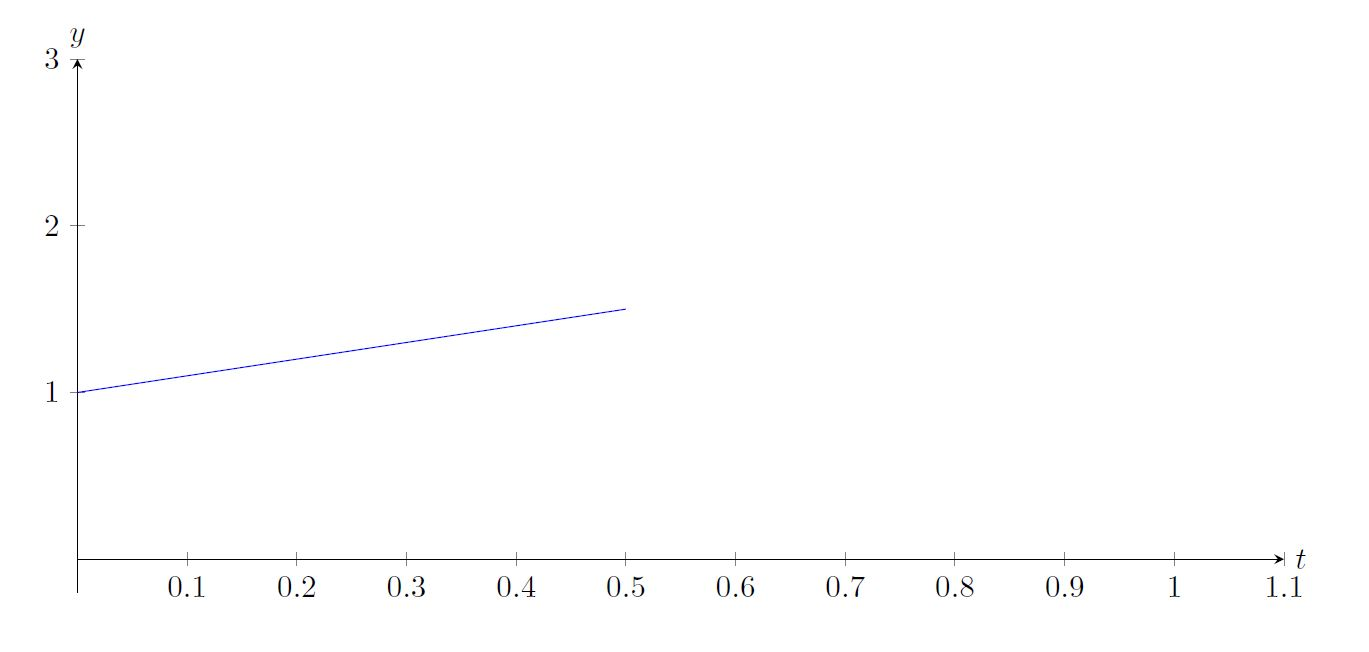
\includegraphics[height=1.5in]{fig030101.jpg} 
\end{image}


% Commented out by Felipe
%\begin{image}
%  \begin{tikzpicture}
%    \begin{axis}[
%        domain=0:1, xmin =0,xmax=1.1,ymax=3,ymin=-.2,
%        width=6in,
%        height=3in,
%        %xticklabels={$1$,$1.5$,$2$, $2.5$, $3$},
%        %% ytick style={draw=none},
%        %% yticklabels={},
%        axis lines=center, xlabel=$t$, ylabel=$y$,
%            every axis y label/.style={at=(current axis.above origin),anchor=south},
%            every axis x label/.style={at=(current axis.right of origin),anchor=west},
%          ]
%          \draw[blue] (0,1)--(0.5, 1.5);
%      %\addplot [blue,very thick] plot coordinates {(0,1) (.5,1.5)};
%    \end{axis}
%\end{tikzpicture}
%\end{image}
But now, we have
$$
y'\left(\frac{1}{2}\right) \approx \frac{1}{2}+\frac{3}{2} = 2
$$
so
$$
y(1) \approx  y\left(\frac{1}{2}\right)+\frac{1}{2} \cdot 2= \frac{5}{2}
$$

\begin{image}
 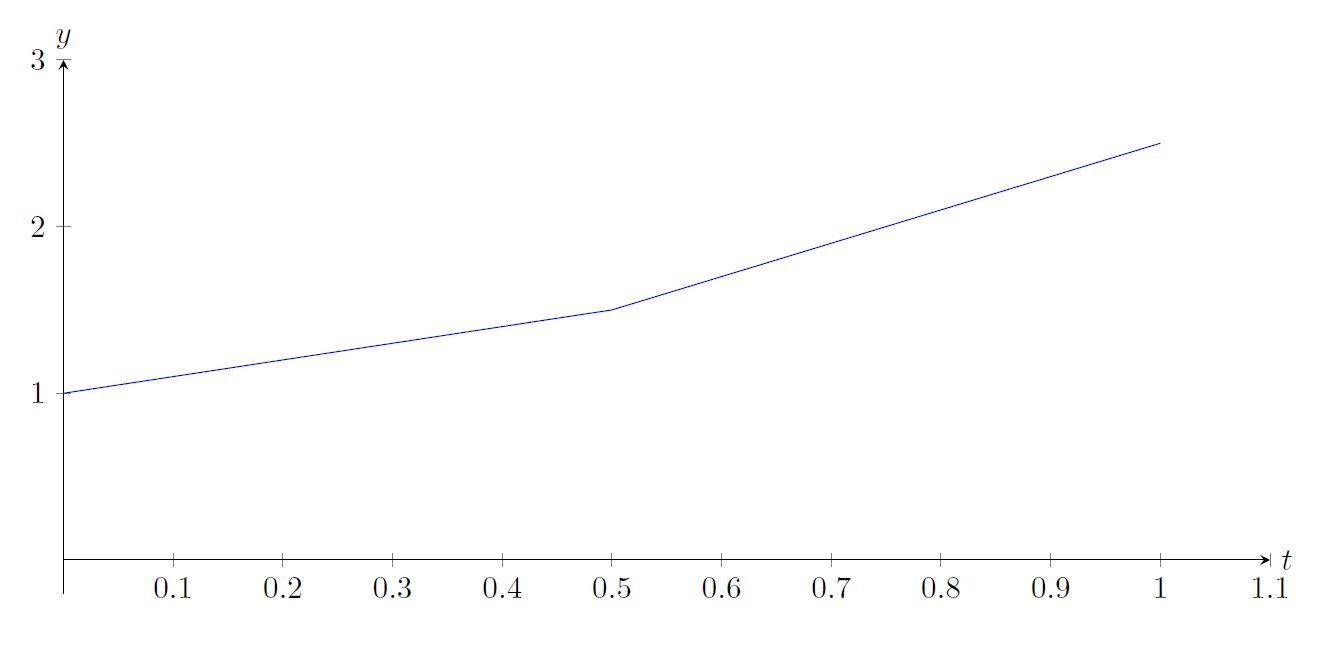
\includegraphics[height=1.5in]{fig030102.jpg} 
\end{image}

% Commented out by Felipe
%\begin{image}
%  \begin{tikzpicture}
%    \begin{axis}[
%        domain=0:1, xmin =0,xmax=1.1,ymax=3,ymin=-.2,
%        width=6in,
%        height=3in,
%        %xticklabels={$1$,$1.5$,$2$, $2.5$, $3$},
%        %% ytick style={draw=none},
%        %% yticklabels={},
%        axis lines=center, xlabel=$t$, ylabel=$y$,
%            every axis y label/.style={at=(current axis.above origin),anchor=south},
%            every axis x label/.style={at=(current axis.right of origin),anchor=west},
%          ]
%        \draw[blue] (0,1)--(0.5, 1.5);
%        \draw[blue] (0.5,1.5)--(1, 2.5);
%      %\addplot [draw=blue,ultra thick] plot coordinates {(0,1) (.5,1.5)};
%      %\addplot [draw=blue,ultra thick] plot coordinates {(.5,1.5) (1,2.5)};
%    \end{axis}
%\end{tikzpicture}
%\end{image}
Plotting our approximation with the actual solution we find:

\begin{image}
 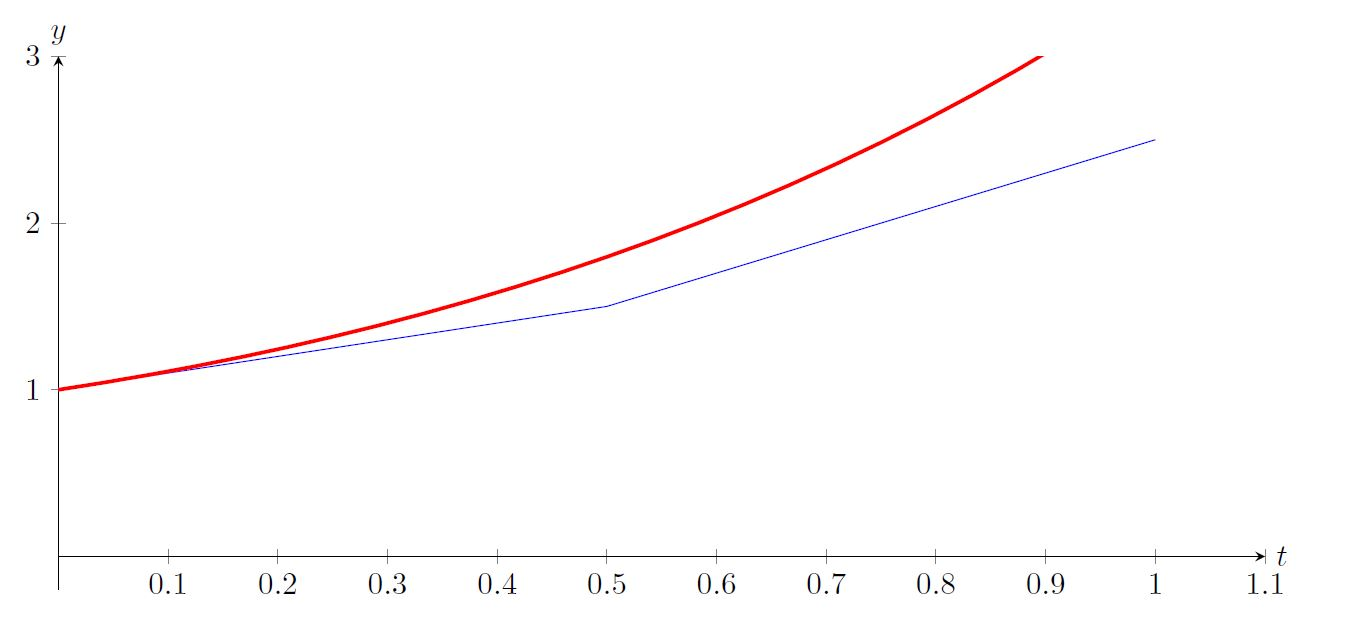
\includegraphics[height=1.5in]{fig030103.jpg} 
\end{image}

% Commented out by Felipe
%\begin{image}
%  \begin{tikzpicture}
%    \begin{axis}[
%        domain=0:1, xmin =0,xmax=1.1,ymax=3,ymin=-.2,
%        width=6in,
%        height=3in,
%        %xticklabels={$1$,$1.5$,$2$, $2.5$, $3$},
%        %% ytick style={draw=none},
%        %% yticklabels={},
%        axis lines=center, xlabel=$t$, ylabel=$y$,
%            every axis y label/.style={at=(current axis.above origin),anchor=south},
%            every axis x label/.style={at=(current axis.right of origin),anchor=west},
%          ]
%      %\addplot [draw=blue,very thick] plot coordinates {(0,1) (.5,1.5)};
%      %\addplot [draw=blue,very thick] plot coordinates {(.5,1.5) (1,2.5)};
%      \draw[blue] (0,1)--(0.5, 1.5);
%      \draw[blue] (0.5,1.5)--(1, 2.5);
%      \addplot [red, very thick] {2*e^x-x-1};
%    \end{axis}
%\end{tikzpicture}
%\end{image}
 
 
This approximation could be improved by using more subintervals.  Use the Sage Cell below to increase the number of subintervals to improve the approximation.
 

%\begin{sageCell}
%@interact
%def _(endPoint=input_box(1, width=5),numberOfIntervals=input_box(1, width=5)):
%    a=var('a')
%    b=function('b')(a)
%    de = diff(b,a) ==  a+b
%    soln = desolve(de, [b, a], ics=[0,1])
%    P3=plot(soln(a), (a, 0, endPoint), color='red')
%
%    from sage.calculus.desolvers import eulers_method
%    x,y = PolynomialRing(QQ,2,"xy").gens()
%    pts=eulers_method(x+y,0,1,endPoint/numberOfIntervals,endPoint-(endPoint/numberOfIntervals),algorithm="none")
%
%    P1 = list_plot(pts)
%    P2 = line(pts)
%
%    (P1+P2+P3).show()
%\end{sageCell}
 
\end{example}
 
%Anna's example
\begin{example}\label{ex:eulerIntro2}
Use Euler's method to approximate $y$ on $[0,1]$ using subintervals of length $0.25$ for
the differential equation
$$
y'=x-y,\quad y(0) = 1
$$

\begin{explanation}
 
Fill out the following table for Euler's method using $4$
subintervals.  Use exact values.
\[
\begin{array}{l|l}
   x & y \\ \hline
   0   & 1 \\
   0.25 & \answer{0.75} \\
   \answer{0.5} & \answer{5/8}  \\
   \answer{0.75} & \answer{19/32} \\
   1 & \frac{81}{128}
\end{array}
\]
Thus $y(1) \approx \answer{81/128}$.

\end{explanation}
\end{example}
 
The Sage Cell below illustrates Example \ref{ex:eulerIntro2} graphically.  You can adjust the number of subintervals to see how the approximation is affected.  You can also change the the interval, just for fun.
 
% Commented out by Felipe
%\begin{sageCell}% Anna
%@interact
%def _(endPoint=input_box(1, width=5),numberOfIntervals=input_box(4, width=5)):
%    a=var('a')
%    b=function('b')(a)
%    de = diff(b,a) ==  a-b
%    soln = desolve(de, [b, a], ics=[0,1])
%    P3=plot(soln(a), (a, 0, endPoint), color='red')
%
%    from sage.calculus.desolvers import eulers_method
%    x,y = PolynomialRing(QQ,2,"xy").gens()
%    pts=eulers_method(x-y,0,1,endPoint/numberOfIntervals,endPoint-(endPoint/numberOfIntervals),algorithm="none")
%   
%    tableOfValues=eulers_method(x-y,0,1,endPoint/numberOfIntervals,endPoint,algorithm="table")
%    P1 = list_plot(pts)
%    P2 = line(pts)
%
%    (P1+P2+P3).show()
%\end{sageCell}
 

 
 
\subsection*{Sources of Error}
 
When using numerical methods we're interested in
computing approximate values of the solution of \eqref{eq:3.1.1} at
equally spaced points $x_0, x_1, \ldots, x_n=b$ in an interval
$[x_0,b]$.
 Thus,
$$
x_i=x_0+ih,\quad i=0,1, \dots,n,
$$
where
$$
h=\frac{b-x_0}{n}.
$$
We'll denote the approximate values of the solution at these points
by $y_0, y_1, \ldots, y_n$;   thus, $y_i$ is an approximation to
$y(x_i)$.
We'll call
$$
e_i=y(x_i)-y_i
$$
the \dfn{error at the $i$th step}. Because of the initial
condition
$y(x_0)=y_0$, we'll always have $e_0=0$. However, in general
$e_i\neq 0$ if $i>0$.
 
We encounter two sources of error
in applying a numerical method to solve an initial value problem:
\begin{itemize}
\item
The formulas defining the method are based on some sort of
approximation. Errors due to the inaccuracy of the approximation are
called \dfn{truncation errors}.
\item
Computers do arithmetic with a fixed number of digits, and therefore
make errors in evaluating the formulas defining the numerical methods.
Errors due to the computer's inability to do exact arithmetic are
called \dfn{roundoff errors}.
\end{itemize}
 
Since a careful analysis of roundoff error is beyond the scope of this
book, we'll consider only truncation errors.
 
\begin{example}\label{example:3.1.2}
Use Euler's method with step sizes $h=0.1$, $h=0.05$, and $h=0.025$ to
find approximate values of the solution of the initial value problem
$$
y'+2y=x^3e^{-2x},\quad y(0)=1
$$
at $x=0, 0.1, 0.2, 0.3, \ldots, 1.0$. Compare these approximate
values
with the values of the exact solution
\begin{equation} \label{eq:3.1.6}
y=\frac{e^{-2x}}{4}(x^4+4),
\end{equation}
which can be obtained by the method of Module 1-B. (Verify.)
 
\begin{explanation}
The table below shows the values of the exact solution
\eqref{eq:3.1.6} at the specified points, and the approximate values of
the solution at these points obtained by Euler's method with step
sizes $h=0.1$, $h=0.05$, and $h=0.025$. In examining this table, keep
in mind that the approximate values in the column corresponding to
$h=.05$ are actually the results of 20 steps with Euler's method. We
haven't listed the estimates of the solution obtained for
$x=0.05, 0.15, \dots $, since there's nothing to compare them with in
the column corresponding to $h=0.1$. Similarly, the approximate values
in the column corresponding to $h=0.025$ are actually the results of
$40$ steps with Euler's method.
 
 
$$
\begin{array}{|c|c|c|c|c|}
\hline
x & h=0.1 & h=0.05 & h=0.025 & \text{Exact}\\ \hline
0.0 & 1.000000000 & 1.000000000 & 1.000000000 & 1.000000000 \\
0.1 & 0.800000000 & 0.810005655 & 0.814518349 & 0.818751221 \\
0.2 & 0.640081873 & 0.656266437 & 0.663635953 & 0.670588174 \\
0.3 & 0.512601754 & 0.532290981 & 0.541339495 & 0.549922980 \\
0.4 & 0.411563195 & 0.432887056 & 0.442774766 & 0.452204669 \\
0.5 & 0.332126261 & 0.353785015 & 0.363915597 & 0.373627557 \\
0.6 & 0.270299502 & 0.291404256 & 0.301359885 & 0.310952904 \\
0.7 & 0.222745397 & 0.242707257 & 0.252202935 & 0.261398947 \\
0.8 & 0.186654593 & 0.205105754 & 0.213956311 & 0.222570721 \\
0.9 & 0.159660776 & 0.176396883 & 0.184492463 & 0.192412038 \\
1.0 & 0.139778910 & 0.154715925 & 0.162003293 & 0.169169104\\
\hline
\end{array}
$$
 
You can see that decreasing the step size
improves the accuracy of Euler's method. For example,
$$
y_{\text{exact}}(1)-y_{\text{approx}}(1)\approx
\left\{\begin{array}{l}
.0293\text{ with }h=0.1,\\
.0144\text{ with }h=0.05,\\
.0071\text{ with }h=0.025.
\end{array}\right.
$$
Based on this scanty evidence, you might guess that the error in
approximating the exact solution at a \textit{fixed value of} $x$ by
Euler's method is roughly halved when the step size is halved. You can
find more evidence to support this conjecture by examining
the table below which lists the approximate values of
$y_{\text{exact}}-y_{\text{approx}}$ at
$x=0.1, 0.2, \dots, 1.0$.
 
$$
\begin{array}{|c|c|c|c|}
\hline
x & h=0.1 & h=0.05 & h=0.025\\ \hline
0.1 & 0.0187 & 0.0087 & 0.0042\\
0.2 & 0.0305 & 0.0143 & 0.0069\\
0.3 & 0.0373 & 0.0176 & 0.0085\\
0.4 & 0.0406 & 0.0193 & 0.0094\\
0.5 & 0.0415 & 0.0198 & 0.0097\\
0.6 & 0.0406 & 0.0195 & 0.0095\\
0.7 & 0.0386 & 0.0186 & 0.0091\\
0.8 & 0.0359 & 0.0174 & 0.0086\\
0.9 & 0.0327 & 0.0160 & 0.0079\\
1.0 & 0.0293 & 0.0144 & 0.0071\\
\hline
\end{array}
$$

\end{explanation}
\end{example}
 
Use the Sage Cell below to explore the error in Example \ref{example:3.1.2} visually by changing the size ($h$) of the subintervals.
 
%Commented out by Felipe
%\begin{sageCell} % Anna
%@interact
%def _(h=input_box(0.1, width=5)):
%    a=var('a')
%    b=function('b')(a)
%    de = diff(b,a) ==  (a^3)*e^(-2*a)-2*b
%    soln = desolve(de, [b, a], ics=[0,1])
%    P3=plot(soln(a), (a, 0, 1), color='red')
%
%    from sage.calculus.desolvers import eulers_method
%    x,y = PolynomialRing(QQ,2,"xy").gens()
%    pts=eulers_method((x^3)*e^(-2*x)-2*y,0,1,h,1-h,algorithm="none")
%
%    P1 = list_plot(pts)
%    P2 = line(pts)
%
%    (P1+P2+P3).show()
%\end{sageCell}
 
%\href{https://docs.google.com/spreadsheets/d/1aE9Nh2VZpG2zJI70yeJpjNZDdxxaqFA8qwoZakjrK-M/edit?usp=sharing}{Spreadsheet}% Paul
 

 
 %%%%%%%%%%%%%%%%%%%%%%%%%%%%%%%%%%% new sections from Trench%%%
 
 \begin{example}\label{example:3.1.3}
The tables below show analogous results
for the nonlinear initial value problem
\begin{equation} \label{eq:3.1.7}
y'=-2y^2+xy+x^2, y(0)=1,
\end{equation}
except in this case we can't solve \eqref{eq:3.1.7} exactly.
The results in the ``Exact'' column were obtained by using a
more accurate numerical method known as the
\href{http://www-history.mcs.st-and.ac.uk/Mathematicians/Runge.html}{Runge}-\href{http://www-history.mcs.st-and.ac.uk/Mathematicians/Kutta.html}{Kutta}
method
 with a small step size. They are
exact to eight decimal places.
The following table shows numerical solutions obtained by Euler's method.
$$
\begin{array}{|c|c|c|c|c|}
\hline
x&
h=0.1&
h=0.05&
h=0.025&
\text{``Exact''}\\ \hline
0.0 & 1.000000000 & 1.000000000 & 1.000000000 & 1.000000000 \\
0.1 & 0.800000000 & 0.821375000 & 0.829977007 & 0.837584494 \\
0.2 & 0.681000000 & 0.707795377 & 0.719226253 & 0.729641890 \\
0.3 & 0.605867800 & 0.633776590 & 0.646115227 & 0.657580377 \\
0.4 & 0.559628676 & 0.587454526 & 0.600045701 & 0.611901791 \\
0.5 & 0.535376972 & 0.562906169 & 0.575556391 & 0.587575491 \\
0.6 & 0.529820120 & 0.557143535 & 0.569824171 & 0.581942225 \\
0.7 & 0.541467455 & 0.568716935 & 0.581435423 & 0.593629526 \\
0.8 & 0.569732776 & 0.596951988 & 0.609684903 & 0.621907458 \\
0.9 & 0.614392311 & 0.641457729 & 0.654110862 & 0.666250842 \\
1.0 & 0.675192037 & 0.701764495 & 0.714151626 & 0.726015790\\
\hline
\end{array}
$$
The following table shows the error in approximate solutions obtained by Euler's method.
$$
\begin{array}{|c|c|c|c|}
\hline
x&
h=0.1&
h=0.05&
h=0.025\\ \hline
0.1 & 0.0376 & 0.0162 &0.0076 \\
0.2 & 0.0486 & 0.0218 &0.0104 \\
0.3 & 0.0517 & 0.0238 &0.0115 \\
0.4 & 0.0523 & 0.0244 &0.0119 \\
0.5 & 0.0522 & 0.0247 &0.0121 \\
0.6 & 0.0521 & 0.0248 &0.0121 \\
0.7 & 0.0522 & 0.0249 &0.0122 \\
0.8 & 0.0522 & 0.0250 &0.0122 \\
0.9 & 0.0519 & 0.0248 &0.0121 \\
1.0 & 0.0508 & 0.0243 &0.0119 \\
\hline
\end{array}
$$

\end{example}


Since we think it's important in evaluating the accuracy of the
numerical methods that we'll be studying in this chapter, we
often include a column listing values of the exact solution of the
initial value problem, even if the directions in the example or
exercise don't specifically call for it. If  quotation marks are
included in the heading, the values were obtained by applying the
Runge-Kutta method in a way that's explained in Section~3.3.
If  quotation marks are not included,  the values were
obtained from a known formula for the solution.
In either case, the values are exact to eight places to the
right of the decimal point.

\subsection*{Truncation Error in Euler's Method}

Consistent with the results indicated in
Tables~\ref{table:3.1.1}--\ref{table:3.1.4}, we'll now show that under
reasonable assumptions on $f$ there's a constant $K$ such that
the error in approximating the solution of the initial value problem
$$
y'=f(x,y),\quad y(x_0)=y_0,
$$
at a given point $b>x_0$ by Euler's method with step size
$h=(b-x_0)/n$ satisfies the inequality
$$
|y(b)-y_n|\leq Kh,
$$
where $K$ is a constant independent of $n$.


There are two sources of error (not counting roundoff) in Euler's
method:
\begin{enumerate}
\item\label{item:3.1.1a} % (1)
The error committed in approximating the integral curve by the tangent
line \eqref{eq:3.1.2} over the interval $[x_i,x_{i+1}]$.
\item\label{item:3.1.1b} % (2)
The error committed in replacing $y(x_i)$ by $y_i$ in
\eqref{eq:3.1.2} and using \eqref{eq:3.1.4} rather than \eqref{eq:3.1.2} to
compute $y_{i+1}$.
 \end{enumerate}

Euler's method assumes that $y_{i+1}$ defined in \eqref{eq:3.1.2}  is
an approximation to $y(x_{i+1})$. We call the error in this
approximation the \dfn{local truncation error at the $i$th step},
and denote it by $T_i$;   thus,
\begin{equation} \label{eq:3.1.8}
T_i=y(x_{i+1})-y(x_i)-hf(x_i,y(x_i)).
\end{equation}
We'll now use
\href{http://www-history.mcs.st-and.ac.uk/Mathematicians/Taylor.html}{Taylor's theorem}
 to estimate $T_i$, assuming for
simplicity that $f$, $f_x$, and $f_y$ are continuous and bounded for
all $(x,y)$. Then $y''$ exists and is bounded on $[x_0,b]$. To see
this, we differentiate
$$
y'(x)=f(x,y(x))
$$
to obtain
\begin{eqnarray*}
y''(x) & = & f_x(x,y(x))+f_y(x,y(x))y'(x)\\
 & = & f_x(x,y(x))+f_y(x,y(x))f(x,y(x)).
\end{eqnarray*}
Since we assumed that $f$, $f_x$ and $f_y$ are bounded, there's
a constant $M$ such that
$$
|f_x(x,y(x))+f_y(x,y(x))f(x,y(x))|\leq M,\quad x_0<x<b,
$$
which implies that
\begin{equation} \label{eq:3.1.9}
|y''(x)|\leq M,\quad x_0<x<b.
\end{equation}
Since $x_{i+1}=x_i+h$, Taylor's theorem implies that
$$
y(x_{i+1})=y(x_i)+hy'(x_i)+\frac{h^2}{2}y''(\tilde x_i),
$$
where $\tilde x_i$ is some number between $x_i$ and $x_{i+1}$.
Since $y'(x_i)=f(x_i,y(x_i))$  this can be written as
$$
y(x_{i+1})=y(x_i)+hf(x_i,y(x_i))+\frac{h^2}{2}y''(\tilde x_i),
$$
or, equivalently,
$$
y(x_{i+1})-y(x_i)-hf(x_i,y(x_i))=\frac{h^2}{2}y''(\tilde x_i).
$$
Comparing this with \eqref{eq:3.1.8} shows that
$$
T_i=\frac{h^2}{2}y''(\tilde x_i).
$$
Recalling \eqref{eq:3.1.9}, we can establish the bound
\begin{equation} \label{eq:3.1.10}
|T_i|\leq \frac{Mh^2}{2},\quad 1\leq i\leq n.
\end{equation}
Although it may be difficult to determine the constant $M$, what is
important is that there's an $M$ such that \eqref{eq:3.1.10} holds.
 We say that the
local truncation error of Euler's method is \dfn{of order} $h^2$,
which we write as $O(h^2)$.

Note that the magnitude of the local truncation error in
Euler's method is determined by the second derivative $y''$ of the
solution of the initial value problem. Therefore
 the local truncation error will be larger where $|y''|$ is large,
or smaller where $|y''|$ is small.

Since the local truncation error for Euler's method is $O(h^2)$, it's
reasonable to expect that halving $h$ reduces the local truncation
error by a factor of $4$. This is true, but
 halving the step size also requires twice as many steps to
approximate the solution at a given point. To analyze the overall
effect of truncation error in Euler's method, it's useful to  derive
an equation relating the errors
$$
e_{i+1}=y(x_{i+1})-y_{i+1}\quad\mbox{and}\quad e_i=y(x_i)-y_i.
$$
To this end, recall that
\begin{equation} \label{eq:3.1.11}
y(x_{i+1})=y(x_i)+hf(x_i,y(x_i))+T_i
\end{equation}
and
\begin{equation} \label{eq:3.1.12}
y_{i+1}=y_i+hf(x_i,y_i).
\end{equation}
Subtracting \eqref{eq:3.1.12} from \eqref{eq:3.1.11} yields
\begin{equation} \label{eq:3.1.13}
e_{i+1}=e_i+h\left[f(x_i,y(x_i))-f(x_i,y_i)\right]+T_i.
\end{equation}
The last term on the right is the local truncation error at the $i$th
step. The other terms reflect the way errors made at {previous
steps} affect $e_{i+1}$. Since $|T_i|\leq Mh^2/2$, we see from
\eqref{eq:3.1.13} that
\begin{equation} \label{eq:3.1.14}
|e_{i+1}|\leq |e_i|+h|f(x_i,y(x_i))-f(x_i,y_i)|+\frac{Mh^2}{2}.
\end{equation}
Since we assumed that $f_y$ is continuous and bounded, the mean
value theorem implies that
$$
f(x_i,y(x_i))-f(x_i,y_i)=f_y(x_i,y_i^*)(y(x_i)-y_i)=f_y(x_i,y_i^*)e_i,
$$
where $y_i^*$ is between $y_i$ and $y(x_i)$. Therefore
$$
|f(x_i,y(x_i))-f(x_i,y_i)|\le R|e_i|
$$
for some constant $R$. From this and \eqref{eq:3.1.14},
\begin{equation} \label{eq:3.1.15}
|e_{i+1}|\leq (1+Rh)|e_i|+\frac{Mh^2}{2},\quad 0\leq i\leq n-1.
\end{equation}
For convenience, let $C=1+Rh$. Since $e_0=y(x_0)-y_0=0$, applying
\eqref{eq:3.1.15} repeatedly yields
\begin{eqnarray}
|e_1| & \leq & \frac{Mh^2}{2}\nonumber\\
|e_2| & \leq & C|e_1|+\frac{Mh^2}{2}\leq (1+C)\frac{Mh^2}{2}\nonumber\\
|e_3| & \leq & C|e_2|+\frac{Mh^2}{2}\leq (1+C+C^2)\frac{Mh^2}{2}\nonumber\\
 & \vdots &\nonumber \\|e_n| & \leq &
C|e_{n-1}|+\frac{Mh^2}{2}\leq (1+C+\cdots+C^{n-1})\frac{Mh^2}{2}.\label{eq:3.1.16}
\end{eqnarray}

Recalling the formula for the sum of a geometric series, we see that
$$
1+C+\cdots+C^{n-1}=\frac{1-C^n}{1-C}=\frac{(1+Rh)^n-1}{Rh}
$$
(since $C=1+Rh$). From this and \eqref{eq:3.1.16},
\begin{equation} \label{eq:3.1.17}
|y(b)-y_n|=|e_n|\leq \frac{(1+Rh)^n-1}{R}\frac{Mh}{2}.
\end{equation}
Since Taylor's theorem implies that
$$
1+Rh<e^{Rh}
$$
(verify),
$$
(1+Rh)^n<e^{nRh}=e^{R(b-x_0)}\quad (\mbox{since }nh=b-x_0).
$$
This and \eqref{eq:3.1.17} imply that
\begin{equation} \label{eq:3.1.18}
|y(b)-y_n|\leq Kh,
\end{equation}
with
$$
K=M\frac{e^{R(b-x_0)}-1}{2R}.
$$
Because of \eqref{eq:3.1.18} we say that the
\href{http://www-history.mcs.st-and.ac.uk/Mathematicians/Euler.html}{global truncation
error of Euler's method is of order} $h$, which we write as $O(h)$.

\subsection*{Semilinear Equations and Variation of Parameters}

An equation that can be written in the form
\begin{equation} \label{eq:3.1.19}
y'+p(x)y=h(x,y)
\end{equation}
with $p\not\equiv0$ is said to be \dfn{semilinear}. (Of course,
\eqref{eq:3.1.19} is linear if $h$ is independent of $y$.) One way to
apply Euler's method to an initial value problem
\begin{equation} \label{eq:3.1.20}
y'+p(x)y=h(x,y),\quad y(x_0)=y_0
\end{equation}
for \eqref{eq:3.1.19} is to think of it  as
$$
y'=f(x,y),\quad y(x_0)=y_0,
$$
where
$$
f(x,y)=-p(x)y+h(x,y).
$$
However, we can also start by applying variation of parameters to
\eqref{eq:3.1.20}, as in Sections~2.1\ and 2.4;   thus, we
write the solution of \eqref{eq:3.1.20} as $y=uy_1$, where $y_1$ is a
nontrivial solution of the complementary equation $y'+p(x)y=0$. Then
$y=uy_1$ is a solution of \eqref{eq:3.1.20} if and only if $u$ is a
solution of the initial value problem
\begin{equation} \label{eq:3.1.21}
u'=h(x,uy_1(x))/y_1(x),\quad u(x_0)=y(x_0)/y_1(x_0).
\end{equation}
We can apply Euler's method to obtain approximate values
$u_0, u_1, \dots, u_n$ of this initial value problem, and then take
$$
y_i=u_iy_1(x_i)
$$
as approximate values of the solution of \eqref{eq:3.1.20}.
We'll call this procedure the
\href{http://www-history.mcs.st-and.ac.uk/Mathematicians/Euler.html}{Euler semilinear method}.

The next two examples show that the Euler and Euler semilinear
methods may yield drastically different results.

\begin{example}\label{example:3.1.4}
In Example~\ref{example:2.1.7} we had to leave the solution of the initial
value
problem
\begin{equation} \label{eq:3.1.22}
y'-2xy=1,\quad y(0)=3
\end{equation}
in the  form
\begin{equation} \label{eq:3.1.23}
y=e^{x^2}\left(3 +\int^x_0 e^{-t^2}dt\right)
\end{equation}
because it was impossible to evaluate this integral exactly in terms
of elementary functions.
Use step sizes $h=0.2$, $h=0.1$, and $h=0.05$ to find approximate
values
of the solution of \eqref{eq:3.1.22} at $x=0, 0.2, 0.4, 0.6,
\dots, 2.0$ by
\begin{enumerate}
\item\label{item:3.1.4a} Euler's method;   
\item\label{item:3.1.4b} the Euler semilinear method.
\end{enumerate}



\begin{explanation}
\ref{item:3.1.4a}
Rewriting \eqref{eq:3.1.22} as
\begin{equation} \label{eq:3.1.24}
y'=1+2xy,\quad y(0)=3
\end{equation}
and applying Euler's method with $f(x,y)=1+2xy$ yields the results
shown in the table below. Because of the large differences
between the estimates obtained for the three values of $h$, it
would be clear that these results are useless even if the ``exact''
values were not included in the table.

$$
\begin{array}{|c|c|c|c|c|}
\hline
x&
h=0.2&
h=0.1&
h=0.05&
\text{``Exact''}\\ \hline
0.0 &  3.000000000 & 3.000000000 & 3.000000000     &   3.000000000 \\
0.2 &  3.200000000 & 3.262000000 &3.294348537      &   3.327851973 \\
0.4 &  3.656000000 & 3.802028800 & 3.881421103     &   3.966059348 \\
0.6 &  4.440960000 & 4.726810214 & 4.888870783     &   5.067039535 \\
0.8 &  5.706790400 & 6.249191282 & 6.570796235     &   6.936700945 \\
1.0 &  7.732963328 & 8.771893026 & 9.419105620     &  10.184923955 \\
1.2 & 11.026148659 &13.064051391 &14.405772067     &  16.067111677 \\
1.4 & 16.518700016 &20.637273893 & 23.522935872    &  27.289392347 \\
1.6 & 25.969172024 &34.570423758 & 41.033441257    &  50.000377775 \\
1.8 & 42.789442120 &61.382165543 & 76.491018246    &  98.982969504 \\
2.0 & 73.797840446 & 115.440048291 & 152.363866569 & 211.954462214 \\
\hline
\end{array}
$$


It's easy to see why Euler's method yields such poor results.
Recall that the constant $M$ in
\eqref{eq:3.1.10} -- which plays an important role in determining the
local truncation error in Euler's method -- must be an upper bound for
the values of the second derivative $y''$ of the solution of the
initial
value problem \eqref{eq:3.1.22} on $(0,2)$. The problem is that $y''$
assumes very large values on this interval. To see this, we
differentiate \eqref{eq:3.1.24} to obtain
$$
y''(x)=2y(x)+2xy'(x)=2y(x)+2x(1+2xy(x))=2(1+2x^2)y(x)+2x,
$$
where the second equality follows again from \eqref{eq:3.1.24}.
Since \eqref{eq:3.1.23} implies that $y(x)>3e^{x^2}$ if $x>0$,
$$
y''(x)>6(1+2x^2)e^{x^2}+2x,\quad x>0.
$$
For example, letting $x=2$ shows that $y''(2)>2952$.

\ref{item:3.1.4b}
Since $y_1=e^{x^2}$ is a solution of the complementary equation
$y'-2xy=0$, we can  apply the Euler semilinear method to
\eqref{eq:3.1.22}, with
$$
y=ue^{x^2}\quad\mbox{and}\quad
u'=e^{-x^2},\quad u(0)=3.
$$
The results listed in the following table are clearly better than
those obtained by Euler's method.

$$
\begin{array}{|c|c|c|c|c|}
\hline
x&
h=0.2&
h=0.1&
h=0.05&
\text{``Exact''}\\ \hline
0.0 &  3.000000000  &   3.000000000 &   3.000000000 &   3.000000000 \\
0.2 &  3.330594477  &   3.329558853 &   3.328788889 &   3.327851973 \\
0.4 &  3.980734157  &   3.974067628 &   3.970230415 &   3.966059348 \\
0.6 &  5.106360231  &   5.087705244 &   5.077622723 &   5.067039535 \\
0.8 &  7.021003417  &   6.980190891 &   6.958779586 &   6.936700945 \\
1.0 & 10.350076600  &  10.269170824 &  10.227464299 &  10.184923955 \\
1.2 & 16.381180092  &  16.226146390 &  16.147129067 &  16.067111677 \\
1.4 & 27.890003380  &  27.592026085 &  27.441292235 &  27.289392347 \\
1.6 & 51.183323262  &  50.594503863 &  50.298106659 &  50.000377775 \\
1.8 &101.424397595  & 100.206659076 &  99.595562766 &  98.982969504 \\
2.0 &217.301032800  & 214.631041938 & 213.293582978 & 211.954462214\\
\hline
\end{array}
$$
\end{explanation}
\end{example}

We can't give a general procedure for determining in advance
whether Euler's method or the semilinear Euler method will produce
better results for a given semilinear initial value problem
\eqref{eq:3.1.19}.
 As a rule of thumb, the Euler semilinear method will
yield better results than Euler's method if $|u''|$ is small on
$[x_0,b]$, while Euler's method  yields better results if $|u''|$
is large on $[x_0,b]$.
 In many cases the results obtained by the two methods don't
 differ appreciably. However, we propose the an intuitive
way to decide which is the better method: Try both methods with
multiple step sizes, as we did in Example~\ref{example:3.1.4},
 and accept the results obtained by the method for
which the approximations change less as the step size decreases.

\begin{example}\label{example:3.1.5}
Applying Euler's method with step sizes $h=0.1$, $h=0.05$, and
$h=0.025$ to the initial value problem
\begin{equation}\label{eq:3.1.25}
y'-2y=\frac{x}{1+y^2},\quad y(1)=7
\end{equation}
on $[1,2]$ yields the results in
the table below. 

$$
\begin{array}{|c|c|c|c|c|}
\hline
x&
h=0.1&
h=0.05&
h=0.025&
\text{``Exact''} \\ \hline
1.0 &  7.000000000 &  7.000000000 &  7.000000000 &  7.000000000\\
1.1 &  8.402000000 &  8.471970569 &  8.510493955 &  8.551744786\\
1.2 & 10.083936450 & 10.252570169 & 10.346014101 & 10.446546230\\
1.3 & 12.101892354 & 12.406719381 & 12.576720827 & 12.760480158\\
1.4 & 14.523152445 & 15.012952416 & 15.287872104 & 15.586440425\\
1.5 & 17.428443554 & 18.166277405 & 18.583079406 & 19.037865752\\
1.6 & 20.914624471 & 21.981638487 & 22.588266217 & 23.253292359\\
1.7 & 25.097914310 & 26.598105180 & 27.456479695 & 28.401914416\\
1.8 & 30.117766627 & 32.183941340 & 33.373738944 & 34.690375086\\
1.9 & 36.141518172 & 38.942738252 & 40.566143158 & 42.371060528\\
2.0 & 43.369967155 & 47.120835251 & 49.308511126 & 51.752229656\\
\hline
\end{array}
$$



Applying the Euler semilinear method
with
$$
y=ue^{2x}\quad\mbox{and}\quad u'=\frac{xe^{-2x}}{1+u^2e^{4x}},\quad
u(1)=7e^{-2}
$$
 yields the results in the table below.
 
 $$
\begin{array}{|c|c|c|c|c|}
\hline
x&
h=0.1&
h=0.05&
h=0.025&
\text{``Exact''} \\ \hline
1.0 &  7.000000000 &  7.000000000 &  7.000000000 &  7.000000000\\
1.1 &  8.552262113 &  8.551993978 &  8.551867007 &  8.551744786\\
1.2 & 10.447568674 & 10.447038547 & 10.446787646 & 10.446546230\\
1.3 & 12.762019799 & 12.761221313 & 12.760843543 & 12.760480158\\
1.4 & 15.588535141 & 15.587448600 & 15.586934680 & 15.586440425\\
1.5 & 19.040580614 & 19.039172241 & 19.038506211 & 19.037865752\\
1.6 & 23.256721636 & 23.254942517 & 23.254101253 & 23.253292359\\
1.7 & 28.406184597 & 28.403969107 & 28.402921581 & 28.401914416\\
1.8 & 34.695649222 & 34.692912768 & 34.691618979 & 34.690375086\\
1.9 & 42.377544138 & 42.374180090 & 42.372589624 & 42.371060528\\
2.0 & 51.760178446 & 51.756054133 & 51.754104262 & 51.752229656\\
\hline
\end{array}
$$
 
Since the latter are clearly less dependent on step size
than the former, we conclude that the Euler semilinear method
is better than Euler's method for \eqref{eq:3.1.25}. This conclusion
is supported by comparing the approximate results obtained by the
two methods with the ``exact'' values of the solution.
\end{example}






\begin{example}\label{example:3.1.6}
Applying Euler's method with step sizes $h=0.1$, $h=0.05$, and
$h=0.025$ to  the initial value problem
\begin{equation}\label{eq:3.1.26}
y'+3x^2y=1+y^2,\quad y(2)=2
\end{equation}
on  $[2,3]$ yields the results in the following table. 

$$
\begin{array}{|c|c|c|c|c|}
\hline
x&
h=0.1&
h=0.05&
h=0.025&
\text{``Exact''} \\ \hline
2.0 &2.000000000 & 2.000000000 & 2.000000000 & 2.000000000 \\
2.1 &0.100000000 & 0.493231250 & 0.609611171 & 0.701162906 \\
2.2 &0.068700000 & 0.122879586 & 0.180113445 & 0.236986800 \\
2.3 &0.069419569 & 0.070670890 & 0.083934459 & 0.103815729 \\
2.4 &0.059732621 & 0.061338956 & 0.063337561 & 0.068390786 \\
2.5 &0.056871451 & 0.056002363 & 0.056249670 & 0.057281091 \\
2.6 &0.050560917 & 0.051465256 & 0.051517501 & 0.051711676 \\
2.7 &0.048279018 & 0.047484716 & 0.047514202 & 0.047564141 \\
2.8 &0.042925892 & 0.043967002 & 0.043989239 & 0.044014438 \\
2.9 &0.042148458 & 0.040839683 & 0.040857109 & 0.040875333 \\
3.0 &0.035985548 & 0.038044692 & 0.038058536 & 0.038072838 \\
\hline
\end{array}
$$


Applying the Euler semilinear method with
$$
y=ue^{-x^3}\quad\mbox{and}\quad u'=e^{x^3}(1+u^2e^{-2x^3}),\quad
u(2)=2e^8
$$
yields the following. 

$$
\begin{array}{|c|c|c|c|c|}
\hline
x&
h=0.1&
h=0.05&
h=0.025&
\text{``Exact''} \\ \hline
2.0 &2.000000000 & 2.000000000 & 2.000000000 & 2.000000000 \\
2.1 &0.708426286 & 0.702568171 & 0.701214274 & 0.701162906 \\
2.2 &0.214501852 & 0.222599468 & 0.228942240 & 0.236986800 \\
2.3 &0.069861436 & 0.083620494 & 0.092852806 & 0.103815729 \\
2.4 &0.032487396 & 0.047079261 & 0.056825805 & 0.068390786 \\
2.5 &0.021895559 & 0.036030018 & 0.045683801 & 0.057281091 \\
2.6 &0.017332058 & 0.030750181 & 0.040189920 & 0.051711676 \\
2.7 &0.014271492 & 0.026931911 & 0.036134674 & 0.047564141 \\
2.8 &0.011819555 & 0.023720670 & 0.032679767 & 0.044014438 \\
2.9 &0.009776792 & 0.020925522 & 0.029636506 & 0.040875333 \\
3.0 &0.008065020 & 0.018472302 & 0.026931099 & 0.038072838 \\
\hline
\end{array}
$$


Noting the close
agreement among the  three columns of the first table (at
least for larger values of $x$) and the lack of any such agreement
among the columns of the second table, we conclude that
Euler's method is better than the Euler semilinear method for
\eqref{eq:3.1.26}. Comparing the results with the exact values
supports this conclusion.
\end{example}

In the next two modules we'll study other numerical methods for
solving initial value problems,  called the
\href{http://www-history.mcs.st-and.ac.uk/Mathematicians/Euler.html}{improved Euler method}, the \dfn{midpoint method},
\href{http://www-history.mcs.st-and.ac.uk/Mathematicians/Heun.html}{Heun's method}
and the
\href{http://www-history.mcs.st-and.ac.uk/Mathematicians/Runge.html}{Runge}-\href{http://www-history.mcs.st-and.ac.uk/Mathematicians/Kutta.html}{Kutta method}.
 If the initial value problem is semilinear as
in \eqref{eq:3.1.19},  we also have the option of using variation of
parameters and then applying the given numerical method to the initial
value problem \eqref{eq:3.1.21} for $u$. By analogy with the terminology
used here, we'll call the resulting procedure
\href{http://www-history.mcs.st-and.ac.uk/Mathematicians/Euler.html}{the improved Euler semilinear method}, the \dfn{midpoint semilinear method},
\href{http://www-history.mcs.st-and.ac.uk/Mathematicians/Heun.html}{Heun's semilinear method} or
\href{http://www-history.mcs.st-and.ac.uk/Mathematicians/Runge.html}{the Runge}-\href{http://www-history.mcs.st-and.ac.uk/Mathematicians/Kutta.html}{Kutta semilinear method}, as
the case may be.

 
 
 
 
 
\section*{Text Source}
\href{https://github.com/mooculus/calculus}{MOOCulus},
\href{https://github.com/mooculus/calculus/blob/a5d5bc54f341b1f3224dde40168188e81032ef65/differentialEquations/digInDifferentialEquations.tex#L1}{Numerical Methods} (CC-BY-NC-SA)
 
Trench, William F., "Elementary Differential Equations" (2013). Faculty Authored and Edited Books \& CDs. 8. (CC-BY-NC-SA)

\href{https://digitalcommons.trinity.edu/mono/8/}{https://digitalcommons.trinity.edu/mono/8/} 
 
\end{document}